\begin{problem}{\#1 (15 points)}
    Use the pumping lemma to show that this language is nonregular:
    \begin{align*}
        \{a^nb^na^n\} &= \{aba,aabbaa,aaabbbaaa,\ldots\}\\
        \{a^nba^n\} &= \{aba,aabaa,aaabaaa,\ldots\}\\
        \{a^nb^{2n} &= \{abb,aabbbb,aaabbbbbb,\ldots\}
    \end{align*}
\end{problem}
\begin{solution}
    \begin{enumerate}
        \item 
        First we assume that $L$ is regular and $n$ is the number of states.\\
        Let $w = a^nb^na^n$. Thus $|w| = 3n \geq n$.\\
        By pumping lemma, let $w = xyz$, where $|xy|\leq n$.\\
        Let $x=a^p,y=a^q,z=a^rb^na^n$, where $p+q+r=n, p\neq 0, q \neq 0, r\neq 0$.\\
        Let $k=2$. Then $xy^2z=a^pa^{2q}a^rb^na^n$.\\
        The number of $a$'s is :$\left( p+2q+r \right)+n=\left( p+q+r \right)+q+n = 2n+q$\\
        Hence, $xy^2z=a^{n+q}b^na^n$. Since $q\neq 0, xy^2z$ is not of the form $a^nb^na^n$.\\
        Thus, $xy^2z$ is not in $L$ making $L$ not regular.
        \item First we assume that $L$ is regular and $n$ is the number of states.\\
        Let $w = a^nba^n$. Thus $|w| = 2n+1 \geq n$.\\
        By pumping lemma, let $w=xyz$, where $|xy|\leq n$.\\
        Let $x=a^p,y=a^q,z=a^rba^n$, where $p+q+r=n,p\neq 0,q\neq 0, r\neq 0$.\\
        Let $k=2$. Then $xy^2z=a^pa^{2q}a^rba^n$.\\
        The number of $a$'s is: $\left( q+2q+r \right)+n=\left( p+q+r \right)+q+n = 2n+q$\\
        Hence, $xy^2z=a^{n+q}ba^n$. Since $q\neq 0, xy^2z$ is not of the form $a^nba^n$.\\
        Thus $xy^2z$ is not in $L$ making $L$ not regular. 
        \item First we assume that $L$ is regular and $n$ is the number of states.\\
        Let $w = a^nb^{2n}$. Thus $|w| = 3n \geq n$.\\
        By pumping lemma, let $w=xyz$, where $|xy|\leq n$.\\
        Let $x=a^p,y=a^q,z=a^rb^{2n}$, where $p+q+r=n,p\neq 0,q\neq 0, r\neq 0$.\\
        Let $k=2$. Then $xy^2z=a^pa^{2q}a^rb^{2n}$.\\
        The number of $a$'s is: $\left( q+2q+r \right)=\left( p+q+r \right)+q = n+q$\\
        Hence, $xy^2z=a^{n+q}b^{2n}$. Since $q\neq 0, xy^2z$ is not of the form $a^nb^{2n}$.\\
        Thus $xy^2z$ is not in $L$ making $L$ not regular.
    \end{enumerate}
\end{solution}

\begin{problem}{\#2 (10 points)}
    By using blue paint, determine which of the following FA's accept any words:
    \begin{enumerate}[label=\alph*)]
        \item 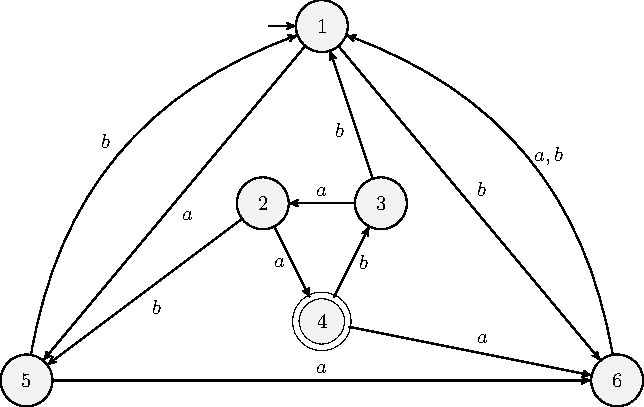
\includegraphics[width=0.7\linewidth]{figures/questions/2a.pdf}
        \item 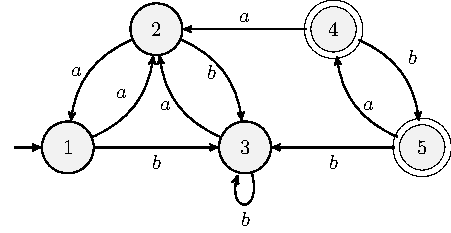
\includegraphics[width=0.6\linewidth]{figures/questions/2b.pdf}
    \end{enumerate}
\end{problem}
\begin{solution}
    \begin{enumerate}
        \item 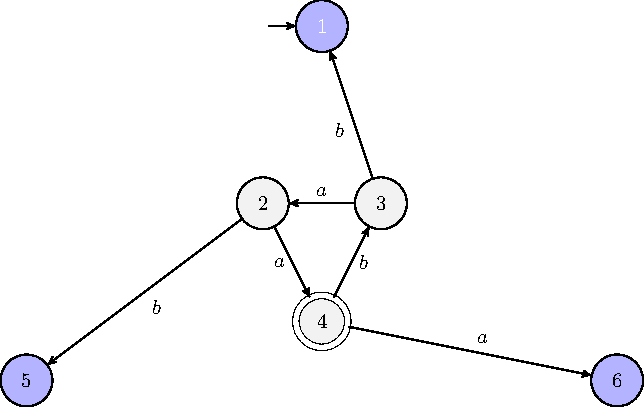
\includegraphics[width=0.7\linewidth]{figures/answers/2a.pdf}
        \item 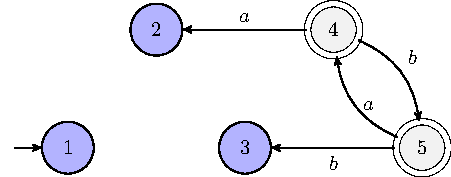
\includegraphics[width=0.6\linewidth]{figures/answers/2b.pdf}
    \end{enumerate}
\end{solution}

\begin{problem}{\#3 (18 points)}
    Describe the language generated by the following context free grammar (CFG) in English and regular expressions:
    \begin{enumerate}[label=\alph*)]
        \item $S \rightarrow SS$\\
        $S \rightarrow ZZZ$\\
        $Z \rightarrow bZ$\\
        $Z \rightarrow Zb$\\
        $Z \rightarrow a$
        \item $S \rightarrow aS$\\
        $S \rightarrow bb$
        \item $S \rightarrow XYX$\\
        $S \rightarrow aX$\\
        $S \rightarrow bX$\\
        $S \rightarrow \Lambda$\\
        $S \rightarrow bbb$
    \end{enumerate}
\end{problem}
\begin{solution}
    
\end{solution}

\begin{problem}{\#4 (15 points)}
    Find CFG for the following languages over the alphabet $\Sigma = \{a,b\}$:
    \begin{enumerate}[label=\alph*)]
        \item All words that have different first and last letters.
        \item All words in which the letter $b$ is never tripled.
        \item All words that do not have substring $ab$.
    \end{enumerate}
\end{problem}
\begin{solution}
    
\end{solution}

\begin{problem}{\#5 (10 points)}
    Show that the CFG below is ambiguous by finding a word with two distinct syntax trees.
    Show both syntax trees.
    \begin{enumerate}[label=\alph*)]
        \item $S \rightarrow Sbb$\\
        $S \rightarrow Sbbb$\\
        $S \rightarrow b$\\
        \item $S \rightarrow AA$\\
        $A \rightarrow AAA|a|bA|Ab$
    \end{enumerate}
\end{problem}
\begin{solution}
    
\end{solution}
